\subsection{Command-Service}
\label{subsec:implementation:commandService}
 Ähnlich wie beim \textit{Query-Service}, wird auch beim \textit{Command-Service} für jeden ankommenden Befehl ein eigener Actor gestartet, der für einen speziellen Typ von Anfrage zuständig ist. Für jeden Typ von Befehl innerhalb der Anwendung gibt es einen Actor welcher die Logik des Befehls beinhaltet. Jedoch werden in der Implementierung der einzelnen Kommandos meist neue Befehle an einen oder mehrere zuständige Actors aus dem Domain-Service erzeugt und weitergeleitet. \\
 In der vorliegenden Implementierung gibt es folgende unterschiedliche Typen von Kommandos, welche alle durch einen \textit{CommandHandler} repräsentiert werden:
 \begin{enumerate}
   \item Flüge erstellen
   \item Flug vorbereiten
   \item Ticket reservieren
   \item Ticket buchen
 \end{enumerate}
Die Abbildung \ref{fig:implementation:commandActorModel} zeigt den Aufbau des \textit{Command-Service}. Die Geschäftslogik ist in den Actors des \textit{Domain Serice} beherbergt. Somit ist die Tätigkeit der einzelnen \textit{CommandHandler} darauf begrenzt, die betroffenen Actors im \textit{Domain Serice} über die gewünschte Tätigkeit zu informieren und diese auszuführen. 
 \begin{figure}
  \centering
  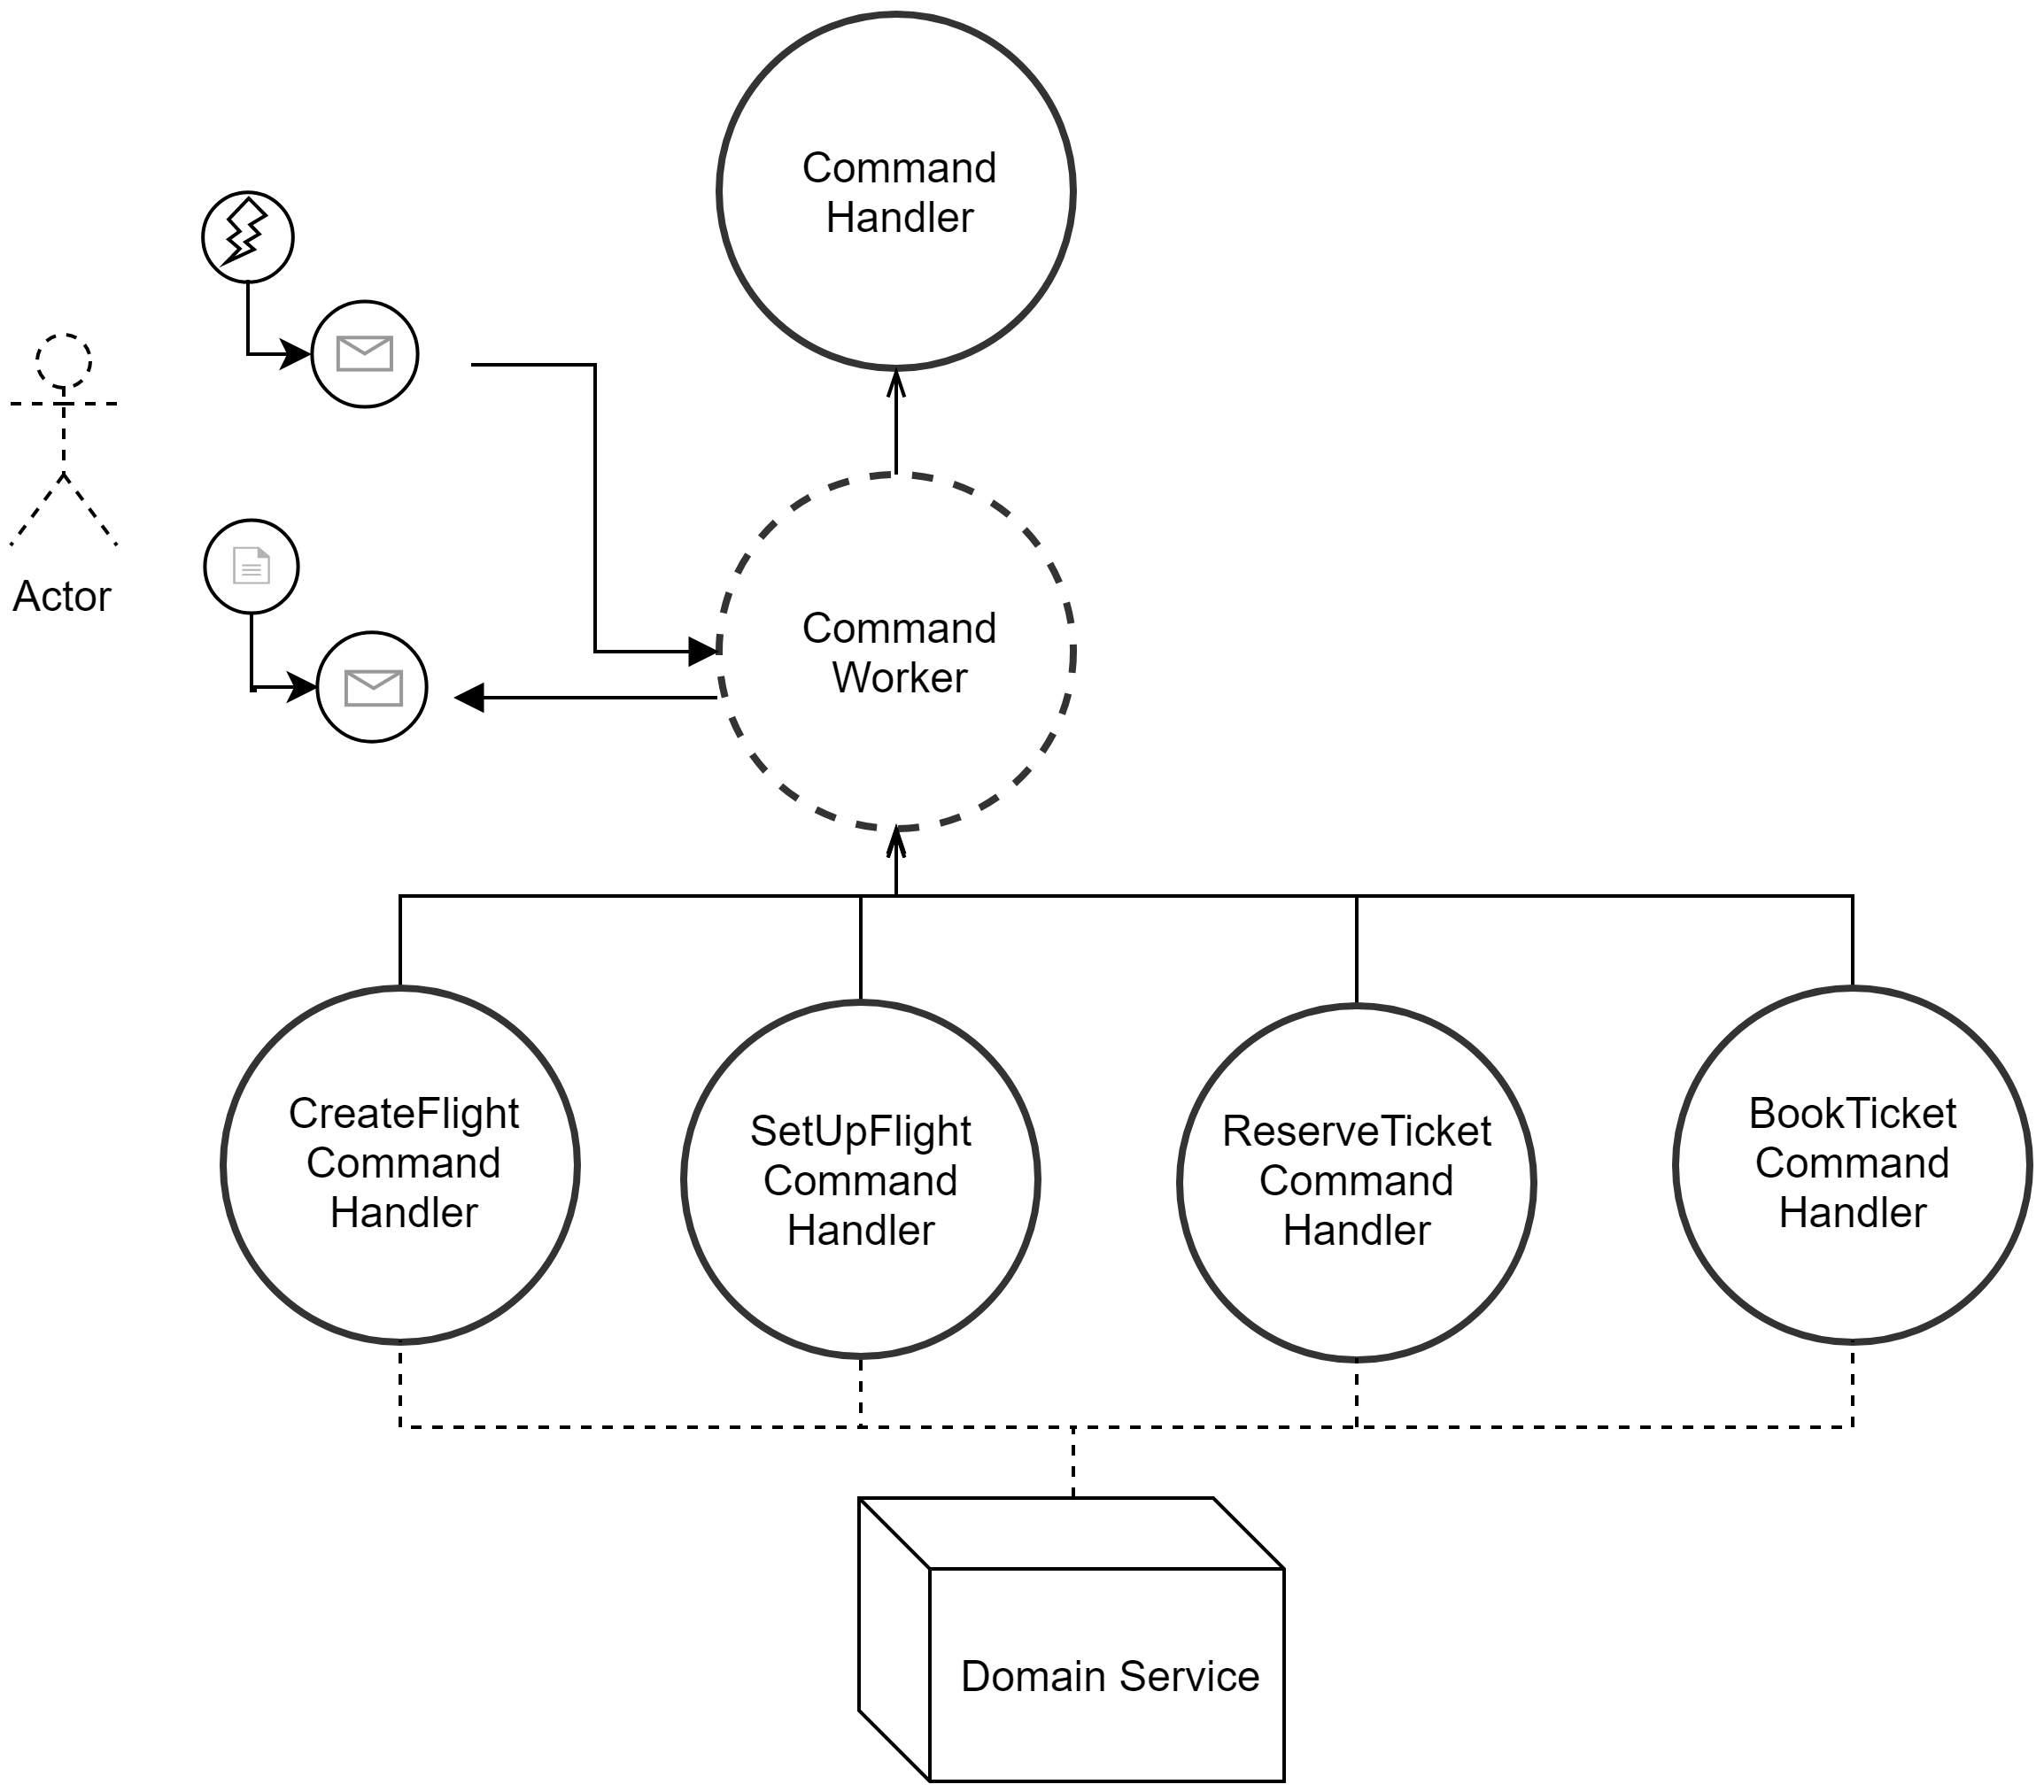
\includegraphics[width=0.8\linewidth]{gfx/implementation/CommandServiceActorModel}
  \caption{Der Aufbau des \textit{Command-Service} beinhaltet die Logik der einzelnen Befehle und leitete weitere Befehle an den \textit{Domain-Service} weiter }
  \label{fig:implementation:commandActorModel}
\end{figure} 

